% Options for packages loaded elsewhere
\PassOptionsToPackage{unicode}{hyperref}
\PassOptionsToPackage{hyphens}{url}
%
\documentclass[
]{article}
\usepackage{lmodern}
\usepackage{amssymb,amsmath}
\usepackage{ifxetex,ifluatex}
\ifnum 0\ifxetex 1\fi\ifluatex 1\fi=0 % if pdftex
  \usepackage[T1]{fontenc}
  \usepackage[utf8]{inputenc}
  \usepackage{textcomp} % provide euro and other symbols
\else % if luatex or xetex
  \usepackage{unicode-math}
  \defaultfontfeatures{Scale=MatchLowercase}
  \defaultfontfeatures[\rmfamily]{Ligatures=TeX,Scale=1}
\fi
% Use upquote if available, for straight quotes in verbatim environments
\IfFileExists{upquote.sty}{\usepackage{upquote}}{}
\IfFileExists{microtype.sty}{% use microtype if available
  \usepackage[]{microtype}
  \UseMicrotypeSet[protrusion]{basicmath} % disable protrusion for tt fonts
}{}
\makeatletter
\@ifundefined{KOMAClassName}{% if non-KOMA class
  \IfFileExists{parskip.sty}{%
    \usepackage{parskip}
  }{% else
    \setlength{\parindent}{0pt}
    \setlength{\parskip}{6pt plus 2pt minus 1pt}}
}{% if KOMA class
  \KOMAoptions{parskip=half}}
\makeatother
\usepackage{xcolor}
\IfFileExists{xurl.sty}{\usepackage{xurl}}{} % add URL line breaks if available
\IfFileExists{bookmark.sty}{\usepackage{bookmark}}{\usepackage{hyperref}}
\hypersetup{
  pdftitle={Perspectives},
  pdfauthor={null},
  hidelinks,
  pdfcreator={LaTeX via pandoc}}
\urlstyle{same} % disable monospaced font for URLs
\usepackage[margin=1in]{geometry}
\usepackage{graphicx}
\makeatletter
\def\maxwidth{\ifdim\Gin@nat@width>\linewidth\linewidth\else\Gin@nat@width\fi}
\def\maxheight{\ifdim\Gin@nat@height>\textheight\textheight\else\Gin@nat@height\fi}
\makeatother
% Scale images if necessary, so that they will not overflow the page
% margins by default, and it is still possible to overwrite the defaults
% using explicit options in \includegraphics[width, height, ...]{}
\setkeys{Gin}{width=\maxwidth,height=\maxheight,keepaspectratio}
% Set default figure placement to htbp
\makeatletter
\def\fps@figure{htbp}
\makeatother
\setlength{\emergencystretch}{3em} % prevent overfull lines
\providecommand{\tightlist}{%
  \setlength{\itemsep}{0pt}\setlength{\parskip}{0pt}}
\setcounter{secnumdepth}{-\maxdimen} % remove section numbering

\title{Perspectives}
\author{null}
\date{null}

\begin{document}
\maketitle

{
\setcounter{tocdepth}{2}
\tableofcontents
}
\emph{Working - needs graphics, formatting, I SUGGEST DELETING TEXT IN
ITALICS}

\hypertarget{models-models-everywhere}{%
\subsection{Models, Models Everywhere}\label{models-models-everywhere}}

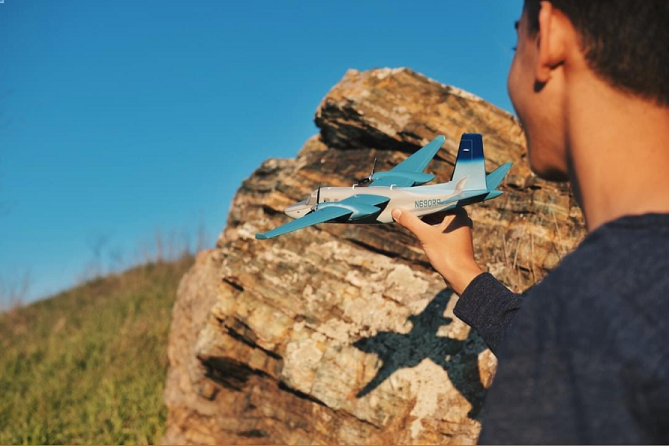
\includegraphics{images/models.png}

Models are everywhere---sometimes behind the scenes and sometimes right
out front. Weather forecasts are models. Measuring the state of the
economy is a model. Assessing the condition of a landscape is a model.
Forecasting almost anything (a pandemic for example) is a model. Many
things we call ``measurements'' are actually models, such as Site Index,
and on and on and on. Even a ``map'' is a model.

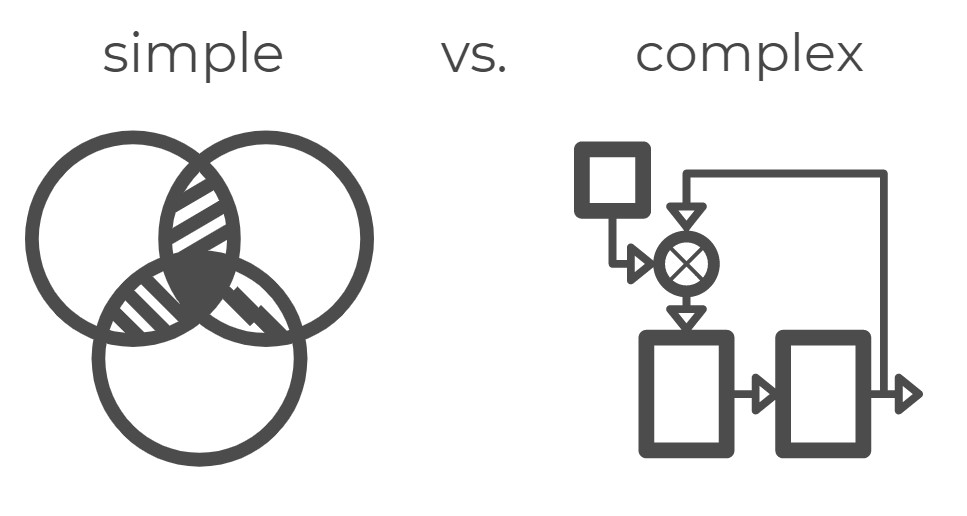
\includegraphics[width=0.45\linewidth]{images/model-simple-vs-complex1}

Regardless of their complexity, ALL models are by definition a
simplification of reality. Like the model airplane shown above\ldots.it
``flies'' like an airplane but it cannot carry cargo or passengers.

\begin{quote}
``All models are wrong, so why do we create and use them?'' - George Box
\end{quote}

We create and use models because (as George Box also said) they can be
useful. In fact, Box used the better word ``illuminating''. Models can
illuminate through prediction or explanation. They can promote
understanding and exploration if used properly. Balance and relevance
are what can make a model illuminating.

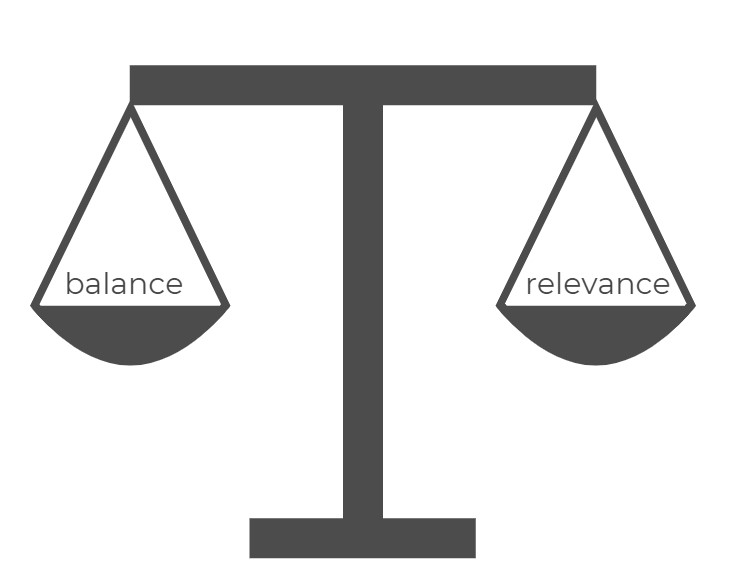
\includegraphics[width=0.55\linewidth]{images/balance-relevance}

\hypertarget{developers-vs-users-key-considerations}{%
\subsection{Developers vs Users: Key
Considerations}\label{developers-vs-users-key-considerations}}

For the model developer, the key is to balance precision and bias of the
outputs with the relevance of the model. The goal is to hit your
application sweet spot.

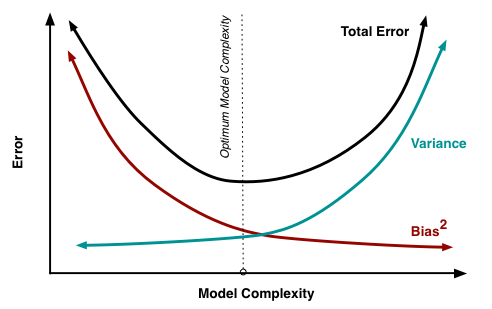
\includegraphics[width=0.55\linewidth]{images/model-complexity}

Image courtesy: \href{francescopochetti.com}{Francesco Pochetti}

The model should provide useful information but must also function for
the user (i.e.~have the right level of complexity). Complexity should
have a purpose: to provide more refined information, or in some cases
provide the same information with more fidelity. Complex models
typically require more input information, are more difficult to develop
and de-bug, and take longer to run.

\begin{quote}
LANDFIRE BpS models, with their limited number of states and
transitions, live near the lower end of the complexity scale and provide
relatively few and coarser level outputs than some other models, but are
also easier to create and use.
\end{quote}

Models such as SIMPPLLE and LANDIS II sit nearer the middle or upper end
of the complexity scale and can provide more types of outputs but at
higher operational cost, sometimes too high a cost.

\hypertarget{understanding-the-characterstics-of-the-model}{%
\subsubsection{Understanding the characterstics of the
model:}\label{understanding-the-characterstics-of-the-model}}

\begin{blue}

\begin{itemize}
\tightlist
\item
  What factors/inputs does it include?
\item
  What factors/inputs does it not include?
\item
  Can you provide the inputs at the level of accuracy required?
\item
  What modeling technique was used?
\item
  How was the model intended to be applied? -What is the ``scale'' of
  the model?
\end{itemize}

\end{blue}

\emph{Like all tools, models can be used correctly or incorrectly. Can a
modified LANDFIRE BpS model provide the information you need with the
right level of quality? Only the user can answer those questions, so it
is imperative that you review the documentation. Communicate with the
modeler if you have questions. It is your responsibility.}

\emph{\#\# Responsibilites}

\emph{Models can be useful and even illuminating if used properly.
Models can be very harmful, unfortunately very obfuscating if used
improperly. It is the modeler's duty to document the model thoroughly
and make that information available to potential users. However, it is
the duty of the model user to know what they really need and to review
the model and model information to decide for themselves if it is
appropriate for their situation or not.}

\textbf{(Does anyone have the picture of Menakis at a RA workshop for
instance---this is not the picture I want to use but collaborative
review is what I want to show) I found the three below in the archives.
Not sure about quality.}

\hypertarget{background-and-recommendations}{%
\subsection{Background and
recommendations}\label{background-and-recommendations}}

\hypertarget{landfire-models}{%
\subsubsection{LANDFIRE Models:}\label{landfire-models}}

LF Biophysical Settings models were created using a set of strict rules
about allowable states (5 or less) and transitions between states (only
historic not current). Key considerations:

\begin{enumerate}
\def\labelenumi{\arabic{enumi}.}
\item
  You are not limited by those rules by the software modeling platform
  (SyncroSim).
\item
  You can add new states and transitions.
\item
  You can modify current states or change transition probabilities.
\item
  If maintaining compatibility with LANDFIRE models is required, your
  modification options may be reduced. However, we have seen STSM based
  on LANDFIRE BpS models that had more than 100 states and dozens of
  transitions.
\item
  LF Biophysical Settings models were developed to reflect the average
  historical dynamics of an Ecological System across an entire NLCD map
  zone or set of NLCD Map Zones (see graphic). That is their ``scale'',
  which may or may not be appropriate for you and your work. If your
  area of interest is significantly larger or smaller that may require
  adjustments to the model.
\end{enumerate}

\textbf{insert Map Zone Map}

\hypertarget{current-condition-model-guide}{%
\subsubsection{Current Condition Model
Guide}\label{current-condition-model-guide}}

\emph{(make this a circular graphic?)}

\begin{enumerate}
\def\labelenumi{\arabic{enumi}.}
\item
  Adhere to established modeling standards.
\item
  Have a goal and a plan. Don't just wing it!
\item
  Work through the model changes in a stepwise fashion. Add states and
  associated transitions one at a time and run the model.
\item
  Review the results and plan the next steps.
\item
  Keep the model as simple as possible. The number of states directly
  impacts the number of transitions you need and the amount of
  information you need to support the model. As the model becomes more
  complicated it becomes more difficult to create, parametrize,
  understand, modify and utilize appropriately.
\item
  Expect the unexpected. If you knew the answer with certainty, you
  probably did not need the model. An answer that seems strange to you
  may be correct, and indeed illuminating.
\end{enumerate}

\end{document}
